\section{Motivație}

Anual se produc peste 8 000 de accidente rutiere grave în România, din care rezultă peste 7 000 de răniți grav și peste 2 000 de persoane decedate. Principalul motiv al tuturor acestor incidente, este de departe reprezentat de erorile umane, de la neatenție sau lipsa de experiență până la oboseală.
\begin{figure}[!h]
	\centering
	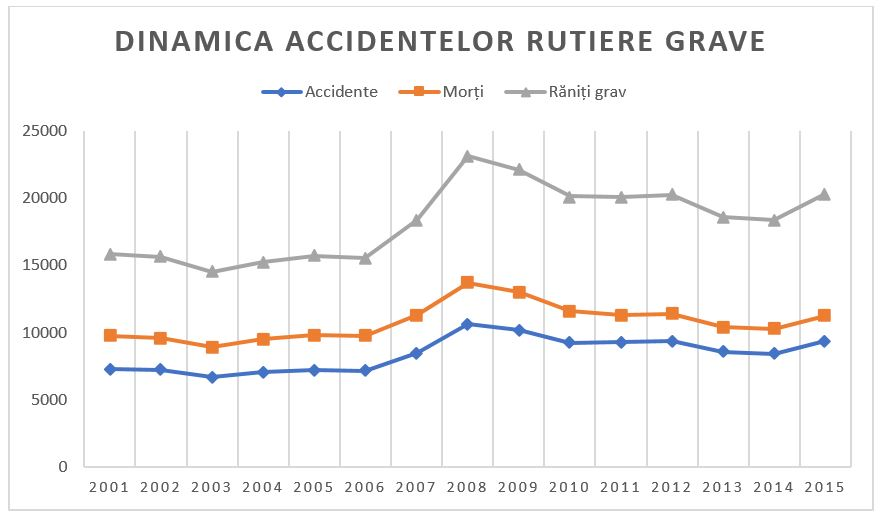
\includegraphics[max width=15cm,max height=15cm,keepaspectratio]{img_1_1}
	\caption{Dinamica accidentelor grave produse în România în perioada 2001 - 2015.}
\end{figure} 

Însă o foarte mare parte a erorilor ce duc la producerea de accidente pot fi evitate cu ajutorul unor sisteme dotate cu inteligență artificială. Sisteme care pot fi de la cele mai elementare lucruri, precum recunoașterea benzii de circulație până la un sistem complet care poate anticipa și preveni anumite evenimente iminente pe care o persoană le-ar sesiza și evita mult mai încet.

Conform raportului $The Atlantic$, accidentele rutiere ar putea fi reduse cu până la $90\%$ în jurul anului 2050 datorită sistemelor de asistență cu care sunt actualele mașini dotate dar și sistemele ce vor fi în dotarea viitoarele generații de mașini.

Abordarea unei teme de actualitate cu implicații majore în prezent și probabil mult mai intense în viitor, abordarea unei teme ce își propune să vină în ajutorul umanității din prisma faptului că poate scădea semnificativ rata accidentelor rutiere produse ca urmare a greșelilor menționate mai sus, au reprezentat principalele motive ale abordării acestei teme.

\section{Obiective propuse}

Prezenta lucrare are drept obiective prinicpale detecția benzii curente de circulație pe care se află mașina, iar pe baza acestei detecții, cautarea eventualei mașinii ce se află pe această bandă. Acestor două obiective principale li se alătură alte două obiective secundare și anume determinarea distanței față de eventuala mașină aflată pe banda detectată și determinarea vitezi relative de deplasare a mașinei curente raportate la mașina detectată ca fiind în fața acesteia pe banda de circulație aferentă.


\section{Structura lucrării}

Prezentarea aplicației realizate debutează prin detalierea fundamentelor teoretice în capitolului II. Aici vom întâlni fundamentele teoretice ce au stat la baza realizării acestei lucrări. Capitolul se deschide prin prezentarea noțiunilor despre vectori suport mașină, un element esențial în antrenarea detectorului de mașini. Pe parcursul acestui capitol vom prezenta noțiunile generale despre vectorii suport mașină, noțiuni despre vectori suport mașină multiclasă dar și vectori suport mașină pentru regresie. 

Vom continua prin a descrie histogramele de gradienți orientați folosite pentru extragerea de caracteristici din imagini. Aceste caracteristici sunt pasate vectorilor suport mașină pentru antrenarea dar sunt folosite ulterior și pentru testarea și validarea potențialelor zone ce conțin mașini. Vor fi prezentate pe lângă noțiunile generale și etapele algoritmului de extragere prin această metodă a caracteristicilor. 

Metoda glisării ferestrei este și ea abordată în fundamentarea teoretică, această metodă este cea care sta la baza identificării zonelor din imagine pentru care detectorul răspunde pozitiv. 

În finalul acestui capitol va fi prezentată noțiunea de IPM, noțiune esențială în detectarea benzii de circulație, pe de o parte, dar și în analiza datelor privind distanța față de mașina aflătă pe banda curentă și de viteza relativă a acesteia în maniera abordată de această lucrare.

Capitolul III este dedicat procesului propriu-zis de dezvoltare al aplicației. Vom începe prin prezentarea componentei ce se ocupă de detectarea benzi. Continuăm prin prezentarea componentei care determină pozițiile eventualelor mașini din imagini și vom incheia prin prezentarea metodelor abordate de detectare a distanței față de mașina din față pe banda curentă de circulație împreună cu viteza relativă în raport cu ea.

Spre finalul lucrării, în capitolul IV, vor fi prezentate bazele de date utilizate atât în cadrul componentei ce se ocupă de detectarea benzii de circulație cât și a componentei ce se ocupă de detectarea de mașini. Pentru fiecare dintre acestea vor fi prezentate informații generale despre respectiva bază de date, tipurile de imagini pe care le conține, algoritmii de evaluare utilizați pentru validarea rezultatelor obținute, dar și rezultatele propriu-zise.

În închierea lucrării vor fi trase concluziile finale și vor fi prezentate posibile viitoare direcții de dezvoltare ale curentei aplicații.

\section{Actualitate}

